\section{Evaluation} \label{sec:evaluation}

\subsection{Unbalanced tree search}

We ran UTS-mem on Grappa and the XMT with a binomial and two geometric
100M-vertex trees and a geometric 1.6B-vertex tree
\footnote{T3L: -t 0 -b 2000 -q 0.200014 -m 5 -r 7\\
          T2L: -t 1 -a 2 -d 23 -b 7 -r 220\\
          T1L: -t 1 -a 3 -d 13 -b 4 -r 29\\
          T1XL: -t 1 -a 3 -d 15 -b 4 -r 29\\}.
Both systems do relatively poorly on the binomial tree because it is very deep and a
traversal produces little parallelism, which both systems depend on.
\TODO{data from our trace would be nice here}. Figure~\ref{fig:grappa-xmt-uts}
shows the performance in terms of number of vertices visited per
second versus number of compute nodes. The Grappa results are for the
best parameter values from a limited search over \flushtimeout~and
\asyncforthr~\TODO{want to say this in general at beginning of eval?}.
Grappa with 16 machines is faster than the entire XMT. Grappa achieves
\checkme{112Mvert/s} with \checkme{60 machines} and the
XMT achieves only 50Mvert/s. Scaling up, Grappa adds 2Mvert/s/nodes
and the XMT adds 850Kvert/s/node. Grappa keeps scaling up through 128
machines, although scaling declines because of the unscalability of our aggregation
mechanism as number of network endpoints increases.


The XMT plataeus around \checkme{60} processors for 100M, 1.6B, and
4.2B-vertex trees, so performance is not limited by availability of
parallelism for this implementation of UTS-mem.


{\em you can rewrite this or blow it off -- just trying to get some thoughts in before leaving}
Despite our efforts to tune the UTS implementation specific to Cray XMT, performance does not scale well with increasing processor count, flattening out around sixty processors.  When we increase the size of the tree, we find that performance does not improve, suggesting that performance is not limited by task parallelism.   Cray's performance tools show that an increasing number of memory retry operations are generated by code within the runtime system.  Retries are performed by the memory controller when remote synchronization operations fail to find the full-bit associated with each memory location in the unavailable state.  Retries are issued at low priority relative to new memory operations issued by the processor by other contexts, so they consume what would otherwise be unused injection bandwidth.  On a full-bandwidth system such as the MTA-2, retries have no impact on the progress of tasks other than their own.  On a Cray XMT, network bandwidth is limited, so retries create congestion.  In comparison, Grappa performs synchronization without retries, delaying response at the receiving end until ready to notify the sender to proceed.  This saves bandwidth and permits scaling of tasks performing synchronization even on low injection rate networks.

\TODO{why is XMT getting different results for T1L,T2L; would expect it to be the machine with the most uniform results.}


\TODO{sensitivity study for \asyncforthr parameter, ie caching amount. Although we can take advantage of locality in children array and the XMT cannot, we still win without it}


\begin{figure}[h]
    \begin{center}
      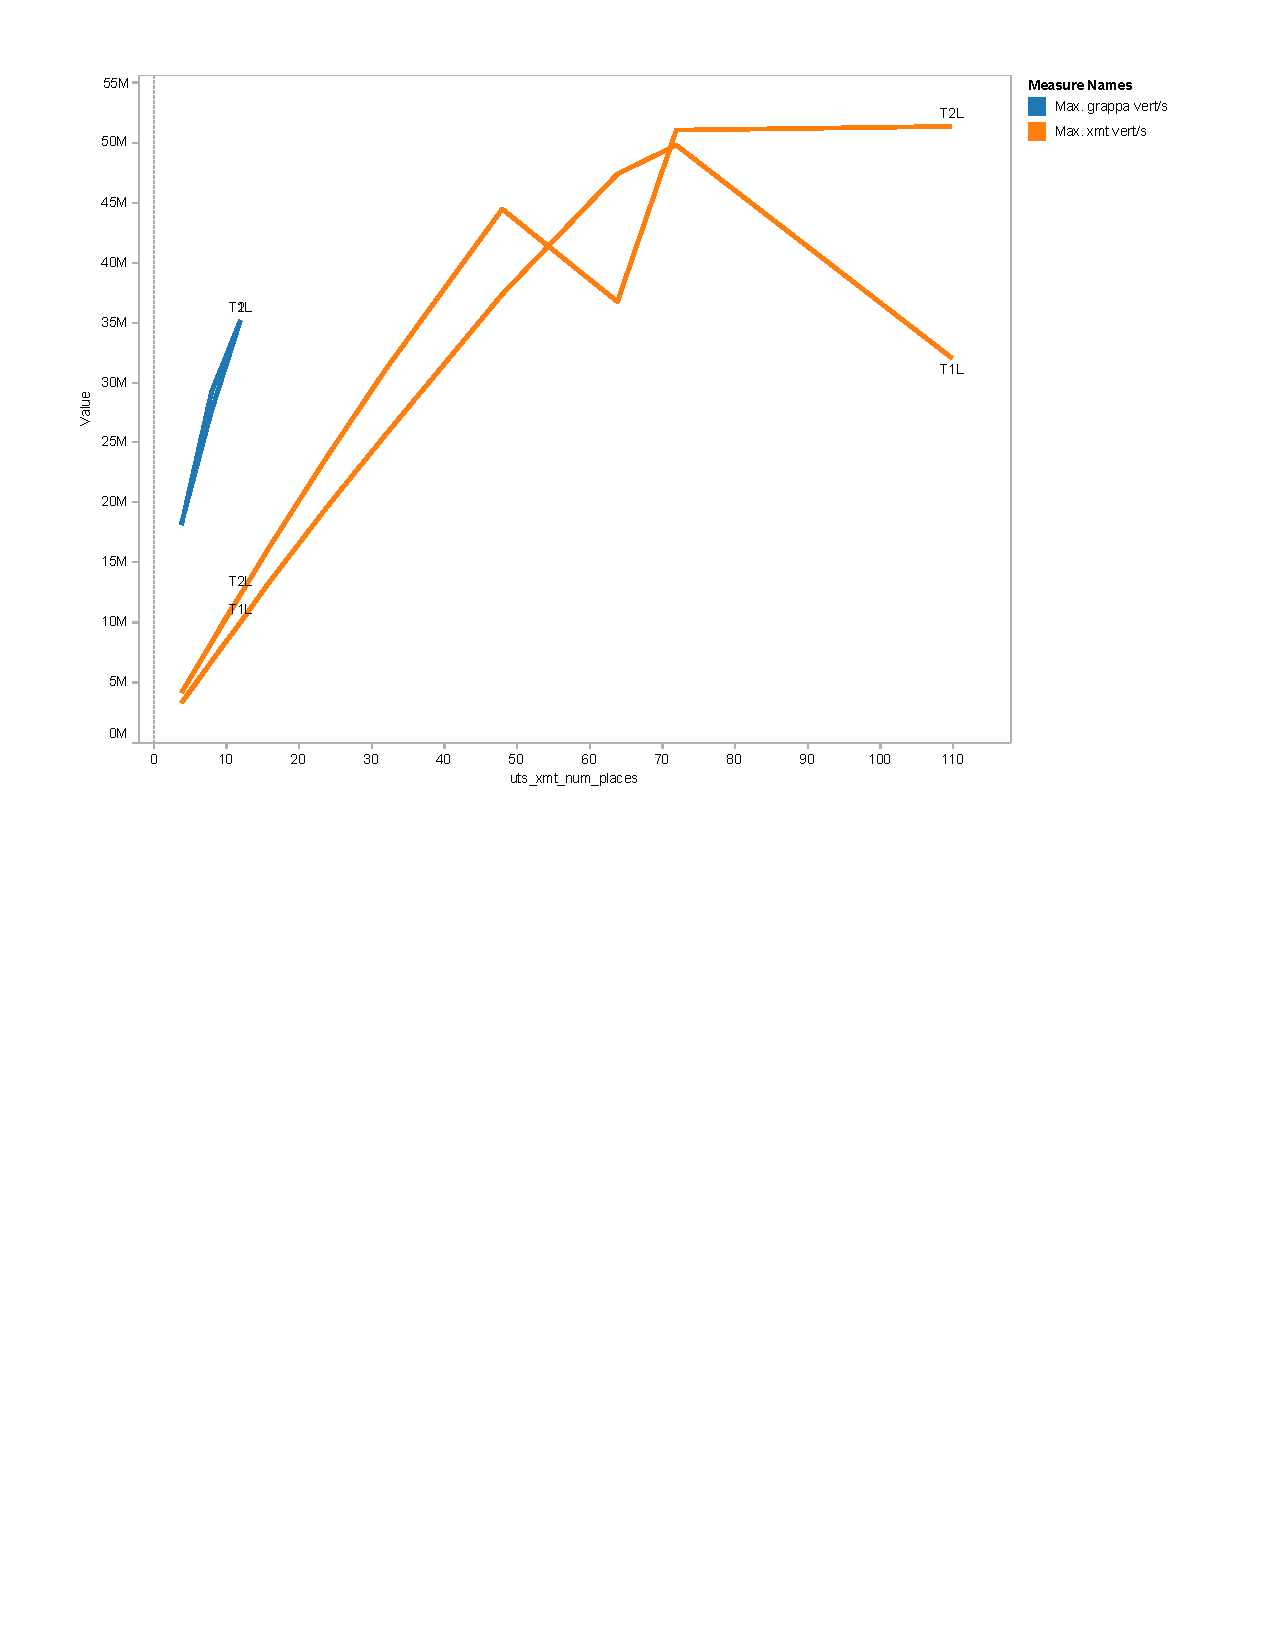
\includegraphics[width=0.5\textwidth]{figs/grappa-xmt-uts.pdf}
    \end{center}
    \caption{describe...}
    \label{fig:grappa-xmt-uts}
\end{figure}






\subsection{Sensitivity}

\subsection{Latency tolerance parameters}

\paragraph{Benefit of aggregator}
what happens with aggregator on and off

\paragraph{Latency}
aggregation latency and delegate latency


\paragraph{Number of workers}
We need enough workers to cover the network+aggregation latency, but more just slow things down.

UTS
BFS


\subsubsection{Work stealing parameters}

\paragraph{Chunk size}

it's important to steal multiple tasks to 
amortize cost of stealing
spread work out quickly in large system

there are times when it's useful to steal lots of stuff, even though
we steal only a few things most of the time.

UTS


\paragraph{Parallel loop threshold}

allows us to amoritize task creation overhead and exploit locality
Gets us a 2x bump in performance
not too sensitive

UTS
BFS



%\begin{figure*}[ht]
%    \begin{minipage}{0.3\linewidth}
%        \centering
%        \includegraphics[width=\textwidth]{figs/chunksize-uts.pdf}
%        \caption{chunksize caption}
%        \label{fig:chunksize-uts}
%    \end{minipage}
%    \begin{minipage}{0.3\linewidth}
%        \centering
%        \includegraphics[width=\textwidth]{figs/workers-uts.pdf}
%        \caption{workers caption}
%        \label{fig:workers-uts}
%    \end{minipage}
%    \begin{minipage}{0.3\linewidth}
%        \centering
%        \includegraphics[width=\textwidth]{figs/thresh-uts.pdf}
%        \caption{threshold caption}
%        \label{fig:thresh-uts}
%    \end{minipage}
%\end{figure*}


Chunksize:
amortizing cost of stealing
spreading work out more
most of the time we still little  (about 10 avg) but sometimes a lot
(difference with BFS)
